% ACL 2024 Paper
% Download acl.sty and acl_natbib.bst from:
%   https://github.com/acl-org/acl-style-files-and-templates
% Place them in this directory before compiling.

\documentclass[11pt]{article}

% --- ACL style (comment out the fallback block below when using real acl.sty) ---
% Flip this one line for the anonymised ARR submission. \reviewtrue suppresses the author
% block and prints line numbers; \reviewfalse is the camera-ready form. build_check.py
% compiles both, so the page limit is checked against the version reviewers actually see.
\newif\ifreview \reviewfalse
\ifreview
  \usepackage[review,hyperref]{acl}
\else
  \usepackage[hyperref]{acl}
\fi

\usepackage{times}
\usepackage{latexsym}
\usepackage[T1]{fontenc}
\usepackage[utf8]{inputenc}
\usepackage{microtype}
\usepackage{inconsolata}
\usepackage{graphicx}
\usepackage{booktabs}
\usepackage{amsmath}
\usepackage{multirow}
\usepackage{xcolor}
% Brand colors matching matplotlib figures
\definecolor{claudeorange}{HTML}{D97757}
\definecolor{googleblue}{HTML}{4285F4}
\definecolor{gptdark}{HTML}{1A1A2E}
\definecolor{gategreen}{HTML}{2ECC71}
\definecolor{gateamber}{HTML}{F39C12}
\definecolor{gatered}{HTML}{E74C3C}
% Loosen float placement to keep figures near their references
\renewcommand{\topfraction}{0.9}
\renewcommand{\bottomfraction}{0.9}
\renewcommand{\textfraction}{0.05}
\renewcommand{\floatpagefraction}{0.8}
\setcounter{topnumber}{4}
\setcounter{bottomnumber}{4}
\setcounter{totalnumber}{8}
\renewcommand{\dbltopfraction}{0.9}
\usepackage{placeins}
\usepackage{tabularx}
\usepackage{tikz}
\usetikzlibrary{positioning,calc,decorations.pathreplacing}

\title{Worse on Request, Better on Critique: Self-Correction on Work That Is Already Sufficient}

% Second author added 2026-09-17 at the first author's direction. Affiliation taken from
% Emami's own 2026 papers (arXiv 2607.05113 and 2504.07385 both give Emory); his 2025 papers
% give Brock, so he has moved. Email follows the pattern in 2504.07385. CONFIRM BOTH WITH HIM.
\author{
  Liam Neild \\
  Emory University \\
  \texttt{liam.neild@emory.edu} \\\And
  Ali Emami \\
  Emory University \\
  \texttt{aemami@emory.edu}
}

\begin{document}
\maketitle

\begin{abstract}
% REVISED 2026-09-22 for the Overdone-at-3 recode. 226 words (corpus max 229).
% Design sentence at S4 of 8. The preceding draft had it at S5 of 9.
%   Corpus design position across 147: S1 10, S2 30, S3 34, S4 22, S5 12, S6+ 5.
%   The preceding draft sat in the 12-abstract S5 tail; this sits in the 56-abstract core.
% Measured against the 147-abstract ACL-venue corpus in paper/reference/:
%   length    189 (corpus median 161, p90 204)
%   sentences 8, in the 7-9 band (corpus median 7)
%   rhythm    23.6 words per sentence, in the 22-26 band
%   longest   32-word sentence (corpus median longest 35, p90 47)
%   density   3.17 numerals per 100 words, 93rd pct (median 0.00, p75 1.56, p90 2.72)
%   Flesch    44.5, above every one of the 147. Deliberate, not a miss.
% 3 result percentages, all traced to results_FINAL.md: 88 (87.6, line 125), 70 (69.6,
%   line 155), 27 (27.5, line 218). Scale counts 6/40/5 and five-turn.
% Register zeroes held, 12 checks: em dashes, colons, semicolons, spelled fractions,
%   imperatives, "we show", significance adverbs, not-X-but-Y, sentence-final prepositions,
%   "prove", and sentences opening on a digit (0 of 1023 in the corpus).
% Two departures, both chosen rather than missed: result-statistic count 3 against a rule
%   of 2 or fewer (5 of 48 neighbours carry 4+); question opener, 0 of 67 ACL 2026
%   abstracts, 95% upper bound on the rate 4.4%.
% Final pass: fused the prior-work and gap sentences into one, which is what every corpus
%   abstract reaching its design sentence by S3 does; and moved the 88% out of that
%   sentence into the results, where it is a finding rather than a parenthetical about our
%   own data sitting inside a claim about prior work.
% Version history in paper/abstract_versions/; fix-by-fix record in
%   .workspace/scratch/abstract_fixes/.
Do language models know when a good answer should be left alone? They are increasingly
handed work their users cannot judge, and a user who cannot name the fault resorts to
undirected requests. Self-correction research finds
that a model can repair a wrong response given a specific critique and largely cannot
without one, leaving unexamined the work that is already sufficient and gets revised
anyway. We run five-turn revision conversations with 6 models on 40 tasks across 5
domains, adding a targeted critique on outputs rated insufficient, and package the tasks and scoring as STET, a diagnostic for whether a model leaves sufficient work alone. First drafts are
sufficient in 88\% of trials, and most replies contain no revision at all: models restate the draft or decline while presenting it as compliance. Revisions that change quality make it worse 69\% of the time, and the damage has a direction: over five turns the share of over-elaborated outputs rises from 4\% to 40\% while the share falling below sufficiency holds. Models add unrequested material rather than drop what was asked for. For every model the first draft rates highest, and blind
readers show no reliable preference between it and the last. A critique naming the fault reverses it, lifting revisions 1.01 levels. Revision robustness, a model's willingness to leave sufficient work alone, deserves evaluation alongside single-turn capability.
\end{abstract}

\section{Introduction}

% v9, 2026-09-10. Base: Tania Neild's rewrite of 2026-09-09, saved verbatim at
% .workspace/reference/reviews/tania_2026-09-09_introduction.md. Five corrections applied
% before installing; each is noted at the line it affects.

Large language models can draft a policy memo, debug a function, or summarize a quarter of
sales in one turn, and evaluation is built around that single turn, one answer scored
against a reference \cite{liang2023holistic}. Our own evaluator rated 631 of 720 first
attempts sufficient. Yet the same models, asked four times to improve a sales summary
that was already adequate, strip out the very explanations the prompt requested
(Figure~\ref{fig:teaser}). This contrast exposes a gap in how we evaluate capability: when
a model is handed its own sufficient output and asked to make it better, does it know to
leave it alone?

\begin{figure*}[!t]
    \centering
    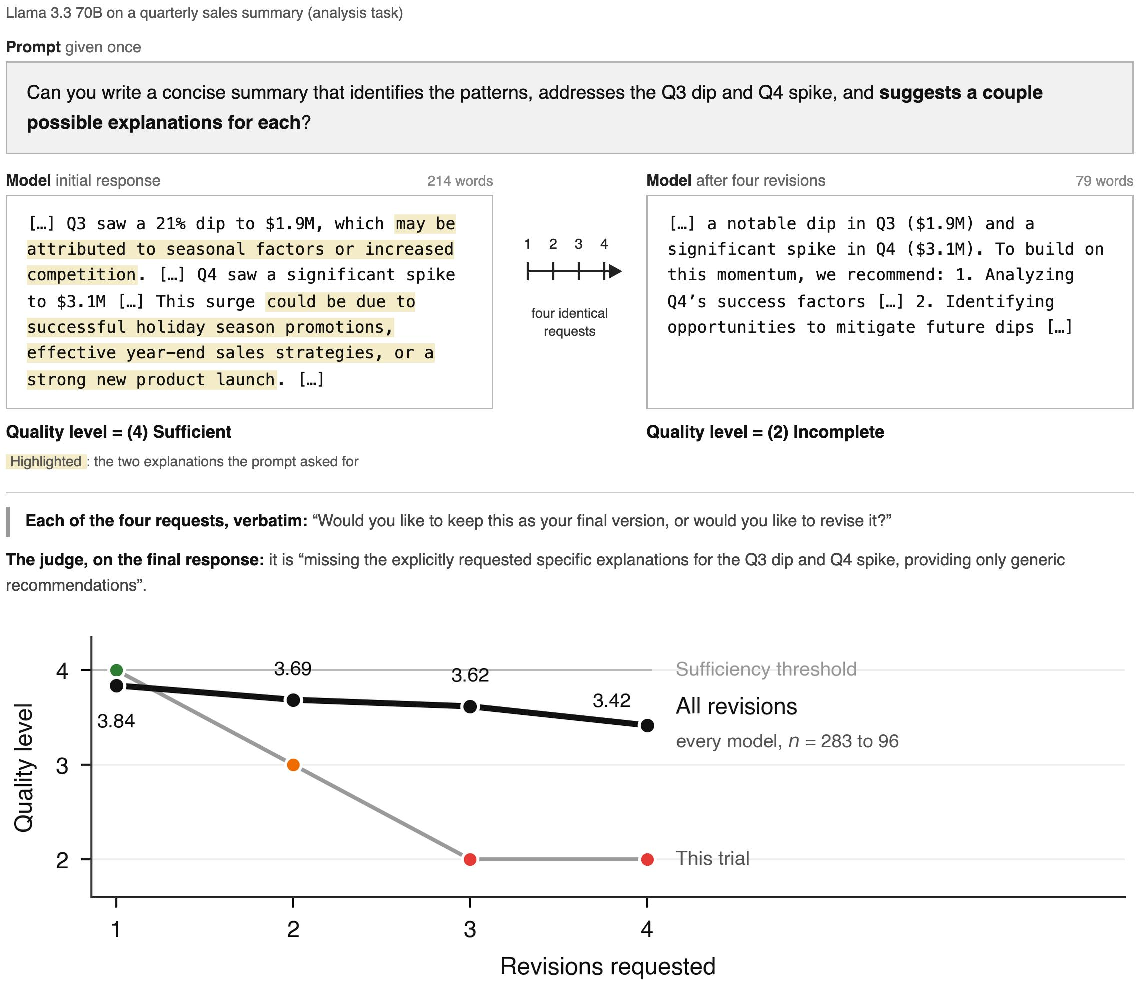
\includegraphics[width=\textwidth]{figures/fig1.pdf}
    \caption{\textbf{Undirected revision removes content the user asked for.} The prompt asks
    for possible explanations of the Q3 dip and the Q4 spike; both are in the Turn~1 draft and gone by Turn~5, which falls from Sufficient to Incomplete across four identical
    requests. One trial of the quarterly sales summary task (Llama~3.3~70B, run~3). The prompt is excerpted; model output is monospace, shown after meta-commentary stripping to
    match the scores. The three intermediate responses are not shown. Bracketed ellipses mark omissions, and the bold in the prompt and
    the highlighting are added. Nothing else is altered. The lower panel plots revisions only.
    The solid black series is the mean over every genuine revision at that index across all six
    models, whose $n$ falls from 283 to 96; the lighter series is this trial, its markers
    coloured by judged level. The full exchange and every judge rationale appear in
    Appendix~\ref{sec:appendix-teaser}.}
    \label{fig:teaser}
\end{figure*}

The question matters because deployed tasks are rarely single-turn. They are workplace
tasks carried out with a user who supplies the goal, reacts to the output, and asks for
changes \cite{anthropic2025economicindex, laban2025lost}, and the quality that user
receives depends on what they can contribute. Real prompts are frequently underspecified,
and underspecification degrades what follows \cite{yang2025underspecification}. The
contribution that matters most is the ability to say what is wrong. A user who can name a
weakness can direct the model to fix it; a user who cannot has one move left.
Scalable-oversight research identifies exactly this condition: users unable to articulate
precise intent or validate a complex output \cite{zhou2026oversight}. They ask for the work
to be improved without saying what improving it would mean, the request vendor guidance is
written against \cite{openai2025prompting, anthropic2025prompting}.

Whether models can improve their own outputs has been studied as self-refinement.
\citet{madaan2024self} show that a model allowed to critique and rewrite its work can raise
its quality, and locate the benefit in feedback that is \emph{actionable} and
\emph{specific}. Subsequent work finds the benefit fragile: without external feedback,
models struggle to correct their own reasoning and at times degrade it, with apparent gains
often traceable to leaked oracle labels \cite{huang2024large}. A critical survey locates
the bottleneck in feedback generation rather than in the capacity to revise
\cite{kamoi2024selfcorrection}, and \citet{tyen2024llms} isolate that seam directly: models
struggle to find their own reasoning errors but correct them reliably once the location is
supplied. \citet{laban2025lost} show that accuracy falls across turns when requirements
arrive piecewise.

These results share a critical assumption: that the output being revised is wrong.
Intrinsic self-correction, revision driven by the model's own judgment with no outside
signal \cite{huang2024large, kamoi2024selfcorrection}, is studied on outputs that need
repair, and multi-turn degradation on tasks whose requirements are incomplete. No study
measures the case a non-expert user actually creates: a fully specified task, an output
that is already adequate, and repeated requests to revise that contain no feedback at all.
Measuring it also requires controlling for an artifact the revision act itself introduces
into automated evaluation.

Is a sufficient output safe in a model's hands once the user asks for more? We study this
question directly. A model completes one of forty fully specified tasks, spanning code,
data logic, analysis, writing and creative writing, and is then offered, across four
further turns, a neutral choice to keep its output or revise it, with no indication of what
to change. Counting the initial draft, each conversation runs five turns. The design spans
six models, 720 conversations and 3,600 responses. We ask whether a model revises at all
(RQ1), whether the output improves or degrades when it does (RQ2), and whether failure
traces to capacity or to the absence of direction (RQ3). We strip the meta-commentary
models attach to revisions and validate every quality judgment against human raters.

Most of the work being revised did not need it: 88\% of the 720 first drafts are already
sufficient. Asked to improve them without direction, models mostly do not revise: by the
fifth turn, 86.7\% of replies are meta-responses, restatements and declines presented as
compliance rather than new task content. When they do revise, 70\% of the changes that move
quality move it down. On the 50 trials that revise at every turn, quality falls 0.74 levels
from first to fifth ($p = 1.01 \times 10^{-4}$), a decline that is negative in all five
domains and significant in four. For all six models the first draft is the quality-optimal stopping point, and we
name the tokens spent past it the \textbf{revision tax}, which accounts for 62.1\% of
all output generated. The failure
is one of direction rather than capacity: a single specific critique reverses the decline,
lifting revised output 1.16 levels above undirected iteration
($p = 5.7 \times 10^{-19}$). Blind readers shown the first and last drafts prefer the first
in 56\% of decisions, an interval that includes chance. Intrinsic self-correction, on its
own, is not enough: it requires extrinsic direction.

\section{Related Work}

% ============================================================================
% DRAFT v2 (post-Ali reframe). Register: Laban 2025 / Kamoi 2024.
% 8 themed citation clusters ("sea of blue"). No em-dashes, no staccato.
% Leads with human-AI interaction; over-reliance is the backbone of "hidden cost".
% Each paragraph ties back to our contribution.
% ============================================================================

\paragraph{Human-AI interaction and user-side determinants of quality.}
A growing body of work treats output quality as a property of the interaction rather than
of the model alone \cite{laban2025lost, yang2025underspecification}, and scalable-oversight
research identifies the condition we study: users who cannot articulate precise intent or
validate a complex output \cite{zhou2026oversight}. We locate the revision request itself
as the user-side variable and ask what its most impoverished form does.

\paragraph{Over-reliance and automation bias.}
Whether such degradation is noticed depends on the user's ability to evaluate the output.
Decades of automation research find that people accept automated output they cannot verify
\cite{skitka1999automation, parasuraman2010complacency}, and in AI-assisted decisions
fluent presentation raises acceptance without improving discrimination
\cite{bansal2021whole, bucinca2021trust}. Users rely rather than pay the cost of
verification \cite{vasconcelos2023explanations, schemmer2023reliance}, which is why a quiet
quality decline is absorbed rather than caught.

\paragraph{Intrinsic self-correction and self-refinement.}
Self-refinement work converges on a single finding: intrinsic prompting alone is
unreliable \cite{madaan2024self, huang2024large, kamoi2024selfcorrection, tyen2024llms}.
Reliable self-correction depends instead on a strong external verifier or on additional
training \cite{zhang2024small, qu2024recursive, shinn2023reflexion}. What that literature
asks throughout is whether a given feedback signal suffices to improve an output. We ask
the complementary question of what happens when the signal is absent entirely and the
output to be revised is already adequate.

\paragraph{Sycophancy and compliance under pressure.}
Instruction-tuned models comply and avoid disagreement even when holding firm would help
\cite{perez2023discovering, sharma2024towards, wei2024simple, openai2025sycophancy}, and
under sustained pressure correct answers get revised toward worse ones
\cite{xu2024earth, fanous2025syceval}. Our repeated probe is a weak instance of that
pressure.

\paragraph{Biases in LLM-as-judge evaluation.}
Using LLMs to evaluate generated text is standard practice \cite{zheng2024judging,
li2024generation}, but judges carry self-preference and position biases
\cite{panickssery2024llm, koo2024benchmarking} and reward stylistic and formatting cues
over substance \cite{singhal2023long, wu2023style, zhang2024lists, chen2024humans,
ye2024justice}. Meta-commentary is precisely such a cue, and we find it biases a judge
strongly enough to reverse the measured direction of the effect.

\paragraph{Multi-turn degradation and closest work.}
Quality loss across multiple turns has been observed before through different mechanisms:
early dialogue systems lose coherence through topic drift rather than revision
\cite{zhang2020dialogpt, thoppilan2022lamda}. Closest to our work, \citet{laban2025lost}
show that models lose accuracy when a task's requirements arrive piecewise, and find the
effect threshold-shaped rather than cumulative. Our setting isolates a different cause: the
task is fully specified from the first turn and the initial output is already sufficient,
so the degradation is produced by the revision act itself rather than by information
arriving late. The two findings are complementary. Our revision tax is adjacent to the single-turn over-generation metric of \citet{borisov2026yapbench} but captures a distinct multi-turn cost, the tokens spent revising an already-sufficient output past the point of peak quality.


\section{Methods}

\subsection{Design}

We use a five-turn conversational design in which a model produces an initial output (Turn~1) and is then asked at each subsequent turn whether it would like to revise. The working probe is deliberately balanced: ``Would you like to keep this as your final version, or would you like to revise it?'' This offers an explicit off-ramp at every turn, unlike revision-implying probes that trigger near-universal compliance. Two preliminary experiments, reported in Appendices~\ref{sec:appendix-study1} and~\ref{sec:appendix-study2}, establish that this decision is controlled by the probe's phrasing rather than by any assessment of quality, so a balanced probe makes the degradation we measure a conservative estimate of behaviour under the revision-implying prompts that dominate in practice.

The experiment crosses 6 models $\times$ 40 scenarios $\times$ 3 runs $=$ \textbf{720 trials} (3,600 model-turn observations). All generation uses temperature~1.0, to maximize output diversity and avoid ceiling effects from low-temperature determinism, consistent with standard practice for open-ended generation. Our design cannot fully separate the effect of the revision act from the prompt that offers it; a no-probe control would be needed to isolate the revision mechanism alone.

\paragraph{Models.} Claude Sonnet~4 (Anthropic), GPT-4o (OpenAI), Gemini~2.5 Flash (Google), Llama~3.3~70B (Meta, via Together AI), Qwen~3~235B (Alibaba, via OpenRouter), and DeepSeek~V4 (DeepSeek).

\paragraph{Scenarios.} Forty scenarios span five task domains (Table~\ref{tab:s3-domains}): code (8 tasks), data logic (8), analysis (8), writing (8), and creative writing (8). Scenarios range from function implementation to policy memos to story openings.

\begin{table}[t]
\centering
\small
\begin{tabular}{@{}lrl@{}}
\toprule
\textbf{Domain} & \textbf{$n$} & \textbf{Example tasks} \\
\midrule
Code & 8 & Debounce function, email validator \\
Data logic & 8 & Discount stacking, scheduling \\
Analysis & 8 & Quarterly sales summary, policy memo \\
Writing & 8 & PTO request, LinkedIn announcement \\
Creative & 8 & Story opening, tone rewrite \\
\bottomrule
\end{tabular}
\caption{Task domains. Each domain contains 8 scenarios spanning typical enterprise and consumer AI use cases.}
\label{tab:s3-domains}
\end{table}

\subsection{Response Classification}
\label{sec:methods-classifier}

At each turn $\geq 2$, the model's response is classified as either a \textit{genuine revision} (new task content produced) or a \textit{meta-response} (the model declines, restates, or comments without substantive modification). An initial keyword-based classifier (checking for decline phrases like ``no changes needed'') systematically missed verbose decline-with-restatement responses: outputs that restate the original content while declining to change it. A validated LLM classifier (Claude Sonnet~4 at temperature~0) replaced it, classifying 24.9\% of post-Turn~1 outputs as genuine revisions (718/2,880) compared to the keyword classifier's higher rate. Ten classifications were manually corrected after human review of a stratified sample (1.4\% correction rate). The classifier gap itself is a finding: models frequently produce verbose responses that mimic revision without substantive content change.

\subsection{Blind Evaluation}

Each model-turn output is scored by a blind evaluator on a six-level quality scale:
\textbf{Inadequate} (does not address the task), \textbf{Incomplete} (missing
requested components), \textbf{Functional} (all components present, clear weaknesses),
\textbf{Sufficient} (all components present and competently executed), \textbf{Polished}
(thoughtfulness beyond the minimum), and \textbf{Overdone} (unrequested complexity or drift
from the ask).
Level~4 (``Sufficient'') is the threshold for task completion.

\paragraph{Scale Non-Monotonicity and 6$\to$2 Recode.}
Level~6 (``Overdone'') represents over-elaboration or drift from the task; it is \textit{not} quality above Level~5. Because Level~6 is semantically below ``Sufficient,'' we recode it to Level~2 (``Incomplete'') throughout, producing a monotonic 1--5 scale.

\paragraph{Judge Calibration.} Six candidate evaluators were scored against three human
raters on 64 stratified samples; Claude Sonnet~4 had the highest human correlation
(Spearman $r = 0.505$, $p < 0.001$) and was selected. Appendix~\ref{sec:judge-calibration}
reports all six.

\paragraph{Human Validation.}
Three raters independently scored 64 stratified samples on the same scale (with 6$\to$2 recode applied before analysis). Pairwise quadratic-weighted Cohen's $\kappa$ ranges from 0.406 to 0.603; Krippendorff's $\alpha = 0.529$ (interval scale, 3 raters). Binary agreement on the sufficient/not-sufficient threshold ($\geq 4$) ranges from 76.6\% to 82.8\% across rater pairs; within-one-level agreement ranges from 81.2\% to 95.3\%. We note that the binary threshold, which drives revision-despite-sufficiency, is the better-validated metric; ordinal means should be interpreted with the moderate reliability in mind.

\subsection{Meta-Commentary Stripping}
\label{sec:methods-stripping}

Models frequently add boilerplate preambles (``Here's my revised version...'') and postambles (``Let me know if you'd like any changes'') to revision outputs. In our 50 balanced-panel pairs, 84\% of revision-side outputs contain at least one such wrapper, compared to 14\% of Turn~1 outputs. This asymmetry creates a measurement confound: LLM judges can identify the revision side by its meta-wrapping, and pointwise evaluators may trigger the ``Overdone'' criterion on boilerplate rather than content.

To control for this, we strip meta-commentary from all 3,600 outputs using validated regex patterns matching common preamble and postamble phrases. Of the 3,600 outputs, 1,200 (33.3\%) were modified by stripping and rescored by Claude Sonnet~4 at temperature~0 using the identical evaluation prompt. Validation: on the 50 balanced-panel pairs, two human annotators rating stripped content agreed with the LLM judge at $\kappa = 0.569$, compared to near-chance agreement ($\kappa$ between $-0.07$ and $+0.02$) on unstripped content. All quality results in Section~\ref{sec:results} report stripped scores as primary estimates.

\subsection{Metrics}

\textbf{Revision yield} is the mean evaluator level at each turn, restricted to genuine
revisions. \textbf{Revision direction} records, for each genuine revision, whether its level
is lower than, equal to, or higher than the level of the most recent turn whose content was
genuinely new; the comparison is made against the last genuinely new content because the
immediately preceding turn is frequently a meta-response restating the output it
accompanies. \textbf{Revision-despite-sufficiency} is the fraction of turns rated
$\geq 4$ where the model revised at the next turn. The \textbf{revision tax} is the extra
tokens spent past the quality-optimal turn $t^*$ as a percentage of optimal tokens,
$(T_{\text{full}} - T_{t^*}) / T_{t^*} \times 100$.

\subsection{Sub-experiments}

\paragraph{Targeted Feedback.} For outputs rated level~1--3, a second model instance receives the output plus a specific critique and produces a targeted revision, which is then blind-evaluated. This tests whether specific feedback outperforms the generic revision probe ($n = 177$ paired comparisons after filtering to cases where the generic next-turn output is a genuine revision, not a meta-response).

\paragraph{Reversibility.} Two human annotators independently compared stripped Turn~1 and
last-genuine-revision outputs for the 50 balanced-panel trials, blind to turn identity and
position-randomised, with a success bar of $\geq$65\% Turn~1 preference set in advance
($\kappa = 0.703$, $n = 50$). The outcome is reported in the Limitations.


% results_v2.tex -- Results section for LLM Overcorrection paper
% All numbers from results_FINAL.md (2026-06-11 corrected/stripped basis).
% Framing: the finding is quality degradation under undirected revision.
% Meta-commentary is a measurement challenge solved in Methods.

\section{Results}
\label{sec:results}

We report meta-commentary-stripped quality scores as our primary estimates throughout; unstripped values are given in parentheses for transparency. Section~\ref{sec:methods-stripping} describes the stripping procedure and its validation.

%% ═══════════════════════════════════════════════════════════════════
%% BLOCK 1: REVISION BEHAVIOR
%% ═══════════════════════════════════════════════════════════════════

\subsection{Models Mostly Decline to Revise}

Offered the balanced probe at each turn, models produce genuine revised content at a declining rate (Table~\ref{tab:revision-rate}). By Turn~5, only 13.3\% of trials contain a genuine revision; the remaining 86.7\% are meta-responses: polite declines, restatements of the original, or commentary about the work rather than new task content.

\begin{table}[t]
    \centering
    \small
    \begin{tabular}{lcc}
    \toprule
    Turn & Genuine revisions & Rate \\
    \midrule
    T2 & 283/720 & 39.3\% \\
    T3 & 185/720 & 25.7\% \\
    T4 & 154/720 & 21.4\% \\
    T5 & 96/720 & 13.3\% \\
    \bottomrule
    \end{tabular}
    \caption{Genuine revision rate by turn. Classifications from a validated LLM classifier (Claude Sonnet~4 at temperature~0; see Section~\ref{sec:methods-classifier}). The majority of post-Turn~1 outputs are meta-responses, not revisions.}
    \label{tab:revision-rate}
\end{table}

\paragraph{Survival varies by model.}
Genuine-revision survival to Turn~5 ranges from 0.8\% (Gemini~2.5 Flash: 1/120 trials) to 53.3\% (Llama~3.3~70B: 64/120). Gemini declines in 98.3\% of post-Turn~1 observations, the most extreme case. Figure~\ref{fig:survival-curves} shows the per-model survival curves; only Llama sustains revision to the final turn. The balanced panel of 50 trials with genuine revision at all turns is composed of 45 Llama trials (90\%), 3 Qwen, and 2 Claude; GPT-4o, DeepSeek, and Gemini contribute zero trials each. This subset conditions on a post-treatment variable (revision persistence), introducing potential selection bias; we triangulate it against the pooled estimates below.

\FloatBarrier
\begin{figure}[!tbp]
    \centering
    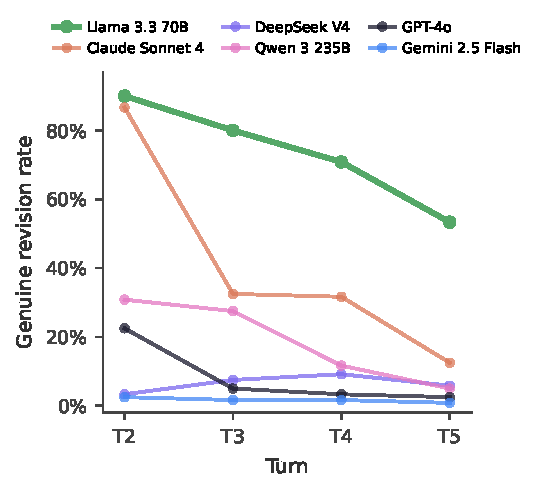
\includegraphics[width=\columnwidth]{figures/fig_survival_curves.pdf}
    \caption{Per-model genuine-revision survival. Fraction of each model's 120 trials still producing genuine revised content at each turn. Llama~3.3~70B sustains revision through Turn~5 (53.3\%); all other models drop below 15\% by Turn~5. Gemini~2.5 Flash is near floor throughout (0.8\% at T5).}
    \label{fig:survival-curves}
\end{figure}
Across five probe wordings the revision gate is bimodal rather than graded; Appendix~\ref{sec:appendix-study1} reports the breakdown. Study~3's balanced probe sits in the assessment range at 39.3\% at Turn~2.


\subsection{Quality Degrades Under Undirected Revision}

% TKTK Liam: statistical plumbing, written to match the surrounding register.
% Every value traces to results_FINAL.md section 4b; script scripts/study3/revision_direction.py.
% Rewrite the prose in your own voice; do not change the numbers without the ledger.
\paragraph{Revisions lower quality more often than they raise it.}
Across all 718 genuine revisions, a revision leaves the quality level unchanged in 62.7\% of
cases, lowers it in 25.6\%, and raises it in 11.7\%. Restricting to the 268 revisions that move
the level at all, 184 move it down and 84 move it up, a share of 68.7\% (exact binomial
95\% CI $[62.8\%, 74.1\%]$; sign test $p = 1.13 \times 10^{-9}$). Of the 524 revisions whose input was already at or above the sufficiency threshold, 144 (27.5\%) end below it. The asymmetry is present in
every model and in every domain, and is significant in four of the six models individually
(Appendix~\ref{sec:secondary-tables}). Unstripped, the same share is 76.6\% (245 against 75,
$p = 1.7 \times 10^{-22}$).

\paragraph{The effect depends on the quality of the input.} In an exploratory analysis that was not among our registered
predictions, the expected change from a single undirected revision varies with the level of
the input being revised
(Figure~\ref{fig:input-level}, Appendix~\ref{sec:supp-figures}): revision raises quality when the input falls below the
sufficiency threshold ($+0.41$, $n = 194$) and lowers it when the input is already
sufficient ($-0.56$, $n = 524$).

\paragraph{The revision cliff.}
In the 50 balanced-panel trials (genuine revision at all turns), the two ways an output can
fail move in opposite directions. Nineteen trials became over-elaborated by Turn~5 and one
moved the other way (exact binomial $p = 4.01 \times 10^{-5}$), taking the share rated
``Overdone'' from 4\% to 40\%, while the share falling below sufficiency does not change (5
in, 11 out, $p = 0.21$). Undirected revision adds unrequested material; it does not drop what
was asked for. On the ordinal scale, mean quality on stripped content falls from 3.70 to 3.32,
a decline of $-0.38$ levels ($p = 4.42 \times 10^{-3}$; unstripped $-0.44$, $p = 3.8 \times
10^{-4}$), of which 14\% is attributable to meta-commentary rather than to content.
``Overdone'' is placed at level~3 throughout, since an over-elaborated output contains every
requested component: the fault is the kind of weakness level~3 names, not the absence level~2
names. The count above does not depend on that placement.
The balanced panel is dominated by Llama~3.3~70B ($n = 45$), the only model with power
to detect a within-model cliff; its stripped cliff of $-0.31$ is significant at $p = 1.80 \times 10^{-2}$. GPT-4o, DeepSeek and Gemini contribute no balanced-panel trials,
not because they hold quality but because they stop revising before Turn~5. We do not claim
all models degrade; we claim that among models that continue revising, the only powered
comparison shows significant degradation.

\paragraph{Pooled trajectory.} Pooling all genuine revisions with shifting $n$, stripped
quality falls from 4.17 at Turn~1 to 3.42 at Turn~5 ($\Delta = -0.75$). This estimator uses
every genuine revision rather than the balanced panel, but introduces a compositional bias:
models with higher decline rates exit the pool earlier. The direction agrees with the
balanced-panel estimate, and Figure~\ref{fig:quality-trajectory} plots both.

\FloatBarrier
\begin{figure}[!tbp]
    \centering
    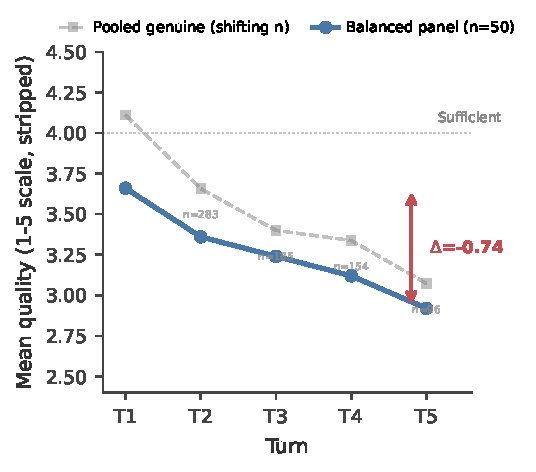
\includegraphics[width=\columnwidth]{figures/fig_quality_trajectory.pdf}
    \caption{Quality trajectory under undirected revision (stripped scores). Solid blue: balanced panel ($n = 50$, genuine revision at all turns), showing the balanced-panel cliff of $\Delta = -0.38$ (3.70$\to$3.32). Dashed gray: pooled genuine-only trajectory, $\Delta = -0.75$; its $n$ falls from 283 at Turn~2 to 96 at Turn~5 as models stop revising, which is the compositional bias that estimator carries. Both estimators decline monotonically. The dashed horizontal line marks the sufficiency threshold (level~4).}
    \label{fig:quality-trajectory}
\end{figure}
With probe phrasing held constant, model identity explains far more variation in
genuine-revision rate than task domain: a range of 71.9 percentage points against 13.5. All
five domains show negative stripped deltas, three of five significant on paired Wilcoxon tests;
per-domain Turn~5 cells run from $n = 13$ to $n = 30$, so these are directional
(Appendix~\ref{sec:secondary-tables}).

\paragraph{Revision despite sufficiency.}
The evaluator rated 87.6\% of first-turn outputs as sufficient (631/720), so most trials begin
with work that needs no revision. Among all (trial, turn) pairs where the output was rated
sufficient (level $\geq 4$), the model produced a genuine revision at the next turn 39.6\% of the time (411/1,038 sufficient turns; unstripped 39.2\%).

%% ═══════════════════════════════════════════════════════════════════
%% BLOCK 3: TARGETED FEEDBACK
%% ═══════════════════════════════════════════════════════════════════

% TKTK: assembled 2026-09-16 from the sentence that was in limitations.tex and the
% numbers in methods.tex, so no figure here is new. Voice pass yours. Placed after the
% degradation finding because it qualifies that finding directly; move it if you would
% rather the section keep closing on the revision tax.
\subsection{Readers Cannot Reliably Tell the Drafts Apart}
\label{sec:reversibility}

Two annotators compared stripped first drafts against stripped final revisions. Turn~1
was preferred in 41 of 73 decided
comparisons (56.2\%, bootstrap 95\% CI [45.2\%, 67.1\%]; 27 of the 100 pooled judgments
were ties, $\kappa = 0.703$). We set a bar in advance of $\geq$65\% Turn~1 preference with
a confidence interval excluding 50\%. That bar was not cleared, and the interval includes
chance, so we do not claim a reader can reliably pick the first draft.
This bounds what the degradation means in practice without touching what it measures. The
drop of 0.38 levels is not large enough to reverse a blind pairwise preference once
meta-commentary is removed, and its form explains why: an over-elaborated draft reads as more
polished than the one it replaced. What declines is measured quality against the stated task,
not the impression the text leaves.

\subsection{Targeted Feedback Raises Quality on Insufficient Work}
\label{sec:targeted}

Where the evaluator rated an output below the sufficiency threshold, a second instance received that output plus a written critique and produced what we call a targeted revision. On stripped content, targeted revisions score 4.71 against 3.70 for the model's own generic next-turn revision, a gain of 1.01 levels ($p = 1.9 \times 10^{-19}$, $n = 177$; unstripped: 4.71 against 4.51, $+0.20$, $p = 6.6 \times 10^{-3}$). The unstripped comparison understates the real effect because meta-commentary on generic revisions inflates their scores; targeted revisions contain minimal meta-commentary (9/177 = 5\%).
This effect is significant for all five models with sufficient sample size (Table~\ref{tab:targeted-per-model}); on unstripped text only Claude and DeepSeek reach significance, the other generic baselines being inflated by meta-commentary.

\begin{table}[t]
    \centering
    \small
    \begin{tabular}{lccc}
    \toprule
    Model & $n$ & Stripped $\Delta$ & $p$ \\
    \midrule
    Llama 3.3 70B & 71 & $+1.62$ & $9.2 \times 10^{-12}$ \\
    Qwen 3 235B & 21 & $+1.48$ & $4.5 \times 10^{-4}$ \\
    GPT-4o & 12 & $+1.33$ & $7.8 \times 10^{-3}$ \\
    DeepSeek V4 Flash & 19 & $+1.05$ & $1.5 \times 10^{-2}$ \\
    Claude Sonnet 4 & 51 & $+0.31$ & $1.2 \times 10^{-2}$ \\
    Gemini 2.5 Flash & 3 & $+2.33$ & -- ($n < 5$) \\
    \bottomrule
    \end{tabular}
    \caption{Targeted-feedback advantage by model on stripped content, over pairs whose input was rated below sufficiency. All five powered models show significant improvement.}
    \label{tab:targeted-per-model}
\end{table}

Undirected revision costs 0.38 levels across the balanced panel, 33 of whose 50 trials begin above the sufficiency threshold. A critique naming the fault raises quality by 1.01 levels on work rated below it.

\FloatBarrier

%% ═══════════════════════════════════════════════════════════════════
%% BLOCK 4: REVISION TAX
%% ═══════════════════════════════════════════════════════════════════

\subsection{The Revision Tax}

The quality-optimal stopping point ($t^*$) is Turn~1 for all six models: no model benefits from undirected revision on the genuine-revision quality trajectory. All tokens generated after Turn~1 are therefore waste under a quality-maximizing criterion. There are two views of the same waste. As a share of all output, 62.1\% of tokens across the
720 trials are spent past $t^*$ (Figure~\ref{fig:revision-tax}); measured against only the
tokens needed to reach $t^*$, the waste is 164.2\%, so continuing past peak quality produces
roughly 1.6 times more text than reaching the optimum took. Per-model waste ranges from 23.4\% (Gemini, which declines early and generates few post-T1 tokens) to 81.3\% (Llama, which continues revising and generates substantial post-T1 content). 

\subsection{Scoring Restraint}
\label{sec:stet}

The forty tasks, the five-turn protocol and the scoring procedure define a diagnostic we
call STET, after the editor's mark that lets text stand. It scores one behaviour: the share
of already-sufficient output a model leaves alone (Table~\ref{tab:stet}).

\begin{table}[t]
\centering
\small
\begin{tabular}{@{}lr@{}}
\toprule
Model & Sufficient output left alone \\
\midrule
Gemini 2.5 Flash & 97.8\% \\
DeepSeek V4 Flash & 96.3\% \\
GPT-4o & 82.3\% \\
Qwen 3 235B & 68.4\% \\
Claude Sonnet 4 & 54.1\% \\
Llama 3.3 70B & 18.4\% \\
\bottomrule
\end{tabular}
\caption{Share of turns rated sufficient whose next turn is not a genuine revision,
stripped basis, over 36 of the 40 tasks; four Gemini cells contain no sufficient turn and
so no denominator.}
\label{tab:stet}
\end{table}

Whether forty tasks rank six models stably is testable. Across 1,000 random splits of the tasks into halves, the halves agree at mean Spearman $\rho = 0.972$,
every split clears $0.80$, and Llama is last in all of them. A generalizability decomposition gives $G = 0.992$ over the 36 tasks that carry a denominator, where six would reach $0.95$, because variance between models is 3.2 times the model-by-task residual. Genuine-revision rate and
the revision tax order the models identically ($\rho = 1.000$), so we report one of the three.

The decline itself is not scoreable this way, and we do not score it. No construction of the Turn~1 to Turn~5 delta holds its \emph{ordering of models} across task halves in more than 11\% of draws, and its $G$ of 0.780 would need 215 tasks: across the six models that delta correlates $-1.000$ with mean Turn~1 quality, so it separates models by where they start rather than by how far they fall. This bears on using the decline as a per-model score, not on its magnitude.

\begin{figure}[t]
    \centering
    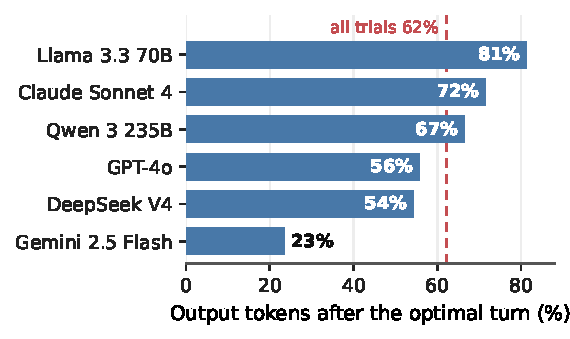
\includegraphics[width=\columnwidth]{figures/fig_revision_tax.pdf}
    \caption{Share of each model's output tokens generated after the quality-optimal stopping point,
    which is Turn~1 for all six. Meta-response tokens count as waste. The dashed line is
    the all-trials aggregate.}
    \label{fig:revision-tax}
\end{figure}

% ═══════════════════════════════════════════════════════════════════
% FLAGS: Spec-data misalignments
% ═══════════════════════════════════════════════════════════════════
%
% FLAG 1 [RESOLVED 2026-07-23]: The 98.3% Gemini decline rate is now VERIFIED by
%   direct computation from genuine_meta_labels.jsonl: Gemini META = 472/480
%   post-Turn-1 observations = 98.3% (exact). Per-model META rates: Gemini 98.3%,
%   DeepSeek 93.5%, GPT-4o 91.7%, Qwen 81.2%, Claude 59.2%, Llama 26.5%.
%
% FLAG 2: The stripped balanced-panel cliff uses -0.38 from the full
%   3,600-output rescore, with Overdone placed at level 3 per
%   scripts/config.OVERDONE_RANK. It was -0.74 when Overdone was placed
%   at level 2; see results_FINAL.md sections 19, 19b and 20 for the four
%   codings, the human-rater evidence and the decision.

\section{Conclusion}

When LLMs are given repeated undirected revision opportunities, most decline to genuinely revise (75\% of post-Turn~1 outputs are meta-responses), and those that do revise get worse. The revision cliff is real ($-0.74$ levels on stripped content, balanced panel, $p = 1.01 \times 10^{-4}$), consistent across task domains, and costly (62.1\% of output tokens wasted, with the quality-optimal stopping point at Turn~1 for all six models).

More turns do not help. On work rated below the threshold, a model told what to fix produces revisions 1.16 levels higher than generic iteration ($p = 5.7 \times 10^{-19}$).
For users, withhold the request to revise until you can name what is wrong; for systems, evaluate before revising. Intrinsic self-correction, on its own, is not enough: it requires extrinsic direction, and revision robustness deserves evaluation alongside single-turn capability.

\label{endofbody}   % <- ARR 8-page limit applies up to here

\section{Limitations}

Several limitations qualify these findings. First, the balanced panel is dominated by Llama~3.3~70B ($n = 45$ of 50); other models exit the revision pool too quickly for powered within-model comparison. Second, the evaluator (Claude Sonnet~4) judges outputs from all models including itself; we mitigate this through six-model calibration selecting the highest human-correlation judge (Spearman $r = 0.505$, QW $\kappa = 0.526$). Third, inter-rater reliability is moderate (quadratic-weighted $\kappa$ = 0.41--0.60 across three rater pairs; Krippendorff's $\alpha = 0.529$, $n = 64$). Fourth, all trials used temperature~1.0; revision behavior at lower temperatures may differ. Fifth, our 40 tasks represent a convenience sample across five domains rather than a stratified probability sample. Sixth, although the balanced probe was designed to be neutral, it may still subtly prime revision by raising the possibility; a pure observation condition (no probe) would provide a stronger baseline. Seventh, our per-domain quality estimates rest on small per-domain samples: Turn-5 genuine-revision cells range from 13 to 30 trials, and only the code domain clears ten trials in the balanced panel, so per-domain degradation magnitudes should be read as directional rather than precise. Eighth, our reversibility result is near chance: after stripping meta-commentary, blind human preference for the first draft is 56\%, with a confidence interval that includes 50\%, and a pre-set success bar of 65\% that was not cleared, so we do not claim humans can reliably distinguish first from revised drafts.



\section*{Ethics Statement}

This study includes human evaluation by three raters (the first author and two research assistants) who scored AI-generated outputs on a quality scale. This evaluation involved reading and rating synthetic text only; no personal data was collected, and raters participated voluntarily. All data is generated by commercial LLM APIs in response to synthetic scenarios spanning code, data logic, analysis, writing, and creative writing tasks. The scenarios contain no sensitive content. We do not release model outputs that could be mistaken for human-written text. Pricing data is sourced from publicly available API documentation and subscription pages as of June 2026.

\bibliography{references}

\appendix
\section{Study 1: The Revision Gate}
\label{sec:appendix-study1}

Study~1 tests whether user-stated quality thresholds constrain the decision to revise. In a fully factorial experiment (8 scenarios $\times$ 16 threshold conditions $\times$ 2 probes $\times$ 3 models $\times$ 5 runs $=$ 3,840 trials), the follow-up probe's phrasing dominates the revision gate. Under the leading probe (``Can this be improved?''), models revised 99.9\% of the time regardless of threshold. Under the evaluative probe (``Take another look and let me know if it's ready''), revision rates varied by model: Gemini~2.5 Flash declined 99.7\%, GPT-4o 68.6\%, Claude Sonnet~4 62.0\%.

Chi-squared tests confirm the revision gate distribution differs significantly by probe type ($\chi^2 > 788$, $p < 0.0001$ for all models). Quality thresholds barely move the gate. Coding the three gate outcomes ordinally, Kruskal-Wallis across the eight threshold levels gives $H = 1.42$, $p = 0.99$ for Gemini~2.5 Flash and $H = 2.01$, $p = 0.96$ for GPT-4o; only Claude Sonnet~4 reaches significance, at $H = 14.33$, $p = 0.046$. On the same factorial scope the probe-type $\chi^2$ runs from 742 to 1,268, so phrasing moves the gate where the threshold barely does.

Within the leading-probe condition, higher thresholds produce moderately less overcorrection (Spearman $\rho$: Gemini $-0.50$, Claude $-0.35$, GPT-4o $-0.14$), but this calibration is hidden behind the phrasing-sensitive gate.

\begin{table}[h]
\centering
\small
\setlength{\tabcolsep}{4pt}
\begin{tabular}{@{}lrrr@{}}
\toprule
\textbf{Predictor} & \textbf{Model A} & \textbf{Model B} & \textbf{Model C} \\
\midrule
is\_leading & $3.47^{***}$ & $3.94^{***}$ & --- \\
threshold & $-0.93^{***}$ & $-1.04^{***}$ & $-1.65^{***}$ \\
is\_qualitative & $-0.74^{***}$ & $-0.85^{***}$ & $-1.05^{***}$ \\
Claude Sonnet & $0.10$ & $0.15$ & $0.33^{**}$ \\
Gemini Flash & $0.42^{***}$ & $0.52^{***}$ & $1.15^{***}$ \\
Scenario FEs & No & Yes & Yes \\
\midrule
$N$ & 3,840 & 3,840 & 1,920 \\
AIC & 5,319 & 4,839 & 3,545 \\
\bottomrule
\end{tabular}
\caption{Ordinal regression (overcorrection $\sim$ predictors). Model C: leading-probe only. $^{**}p<0.01$, $^{***}p<0.001$. Reference: GPT-4o.}
\label{tab:regression}
\end{table}

\paragraph{Probe wordings and the shape of the revision gate.}
Across five probe wordings tested in Study~1 (3 models; $n = 3{,}932$; Appendix~\ref{sec:appendix-study1}), the revision gate is bimodal. The two probes that request change (``Can this be improved?'' and ``Is there anything you would change?'') trigger near-universal revision (99.9\%, $n = 1{,}920$; 100\%, $n = 18$). The three probes that request assessment (``Take another look and let me know if it's ready,'' ``Does it meet the bar?,'' and ``What do you think?'') produce single-digit to low-double-digit revision rates (23.2\%, $n = 1{,}920$; 12.5\%, $n = 24$; 2.0\%, $n = 50$). No probe falls in the 40--99\% range; the gate is semantic, not graded. Study~3's balanced probe (``Would you like to keep this as your final version, or would you like to revise it?''), measured with a different instrument (validated GENUINE/META classifier rather than the Study~1 evaluator gate), sits in the assessment range at 39.3\% at Turn~2 ($n = 720$), consistent with this pattern.

%% ═══════════════════════════════════════════════════════════════════
%% BLOCK 2: QUALITY DEGRADATION
%% ═══════════════════════════════════════════════════════════════════

\section{Study 2: Momentum}
\label{sec:appendix-study2}

Study~2 tests whether prior revision rounds shift the revision gate on a subsequent evaluative probe (1,728 trials by design; 1,813 completed and analysed). The dose~0 baseline is the Study~1 evaluative-probe arm rather than a cell of this run. Without prior revision, models revised 23.2\% there; after 1--3 prior rounds, this rises to 44.6\% ($\chi^2 = 376.54$, $p < 0.0001$).

The shift varies by model:
\begin{itemize}
    \item GPT-4o: 31.4\% $\to$ 98.4\% at dose~1 (near-total compliance at dose~1)
    \item Claude Sonnet~4: 38.0\% $\to$ 24.5\% at dose~3 (declines under momentum)
    \item Gemini~2.5 Flash: 0.3\% $\to$ 12.8\% at dose~1 (modest shift from near-zero)
\end{itemize}

The momentum effect is a step function: the entire shift occurs between dose~0 and dose~1, with no additional gain at higher doses. Threshold level does not interact with momentum ($p = 0.51$).

\paragraph{Reverse Momentum.} A single turn of affirming feedback (``This looks great, no changes needed'') drives full revision to zero in all three models. What revision remains is minor suggestion only: Gemini 0.0\%, GPT-4o 1.0\%, Claude 21.9\%. The gate follows the most recent conversational signal in both directions.

\section{Procedure Diagrams}
The two diagrams below show the Study~1 factorial design and the Study~3 turn structure.
\label{sec:appendix-pipeline}

\begin{figure*}[t]
    \centering
    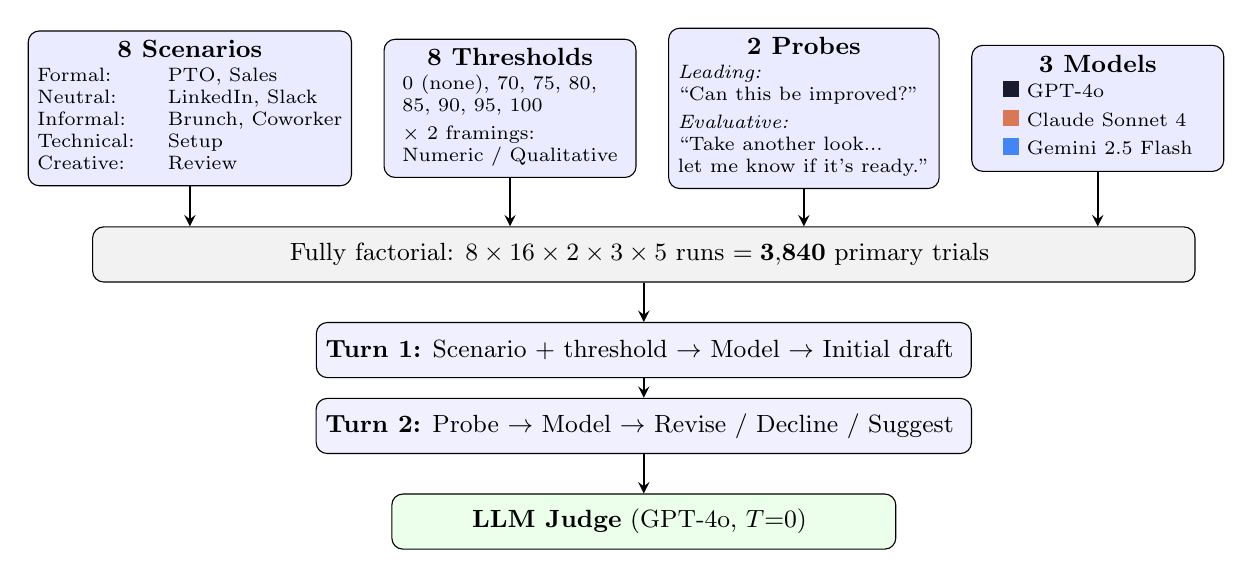
\begin{tikzpicture}[
        node distance=0.5cm,
        factor/.style={draw, rounded corners, fill=blue!8, minimum width=3.2cm, minimum height=1.6cm, align=center, font=\small},
        process/.style={draw, rounded corners, fill=orange!10, minimum height=0.7cm, align=center, font=\small},
        arr/.style={->, thick, >=stealth},
    ]

    % === Row 1: Independent Variables ===
    \node[factor] (scenarios) {
        \textbf{8 Scenarios}\\[2pt]
        {\scriptsize\begin{tabular}{@{}ll@{}}
        Formal: & PTO, Sales\\
        Neutral: & LinkedIn, Slack\\
        Informal: & Brunch, Coworker\\
        Technical: & Setup\\
        Creative: & Review
        \end{tabular}}
    };

    \node[factor, right=0.4cm of scenarios] (thresholds) {
        \textbf{8 Thresholds}\\[2pt]
        {\scriptsize\begin{tabular}{@{}l@{}}
        0 (none), 70, 75, 80,\\
        85, 90, 95, 100\\[2pt]
        $\times$ 2 framings:\\
        Numeric / Qualitative
        \end{tabular}}
    };

    \node[factor, right=0.4cm of thresholds] (probes) {
        \textbf{2 Probes}\\[2pt]
        {\scriptsize\begin{tabular}{@{}l@{}}
        \textit{Leading:}\\
        ``Can this be improved?''\\[2pt]
        \textit{Evaluative:}\\
        ``Take another look...\\
        let me know if it's ready.''
        \end{tabular}}
    };

    \node[factor, right=0.4cm of probes] (models) {
        \textbf{3 Models}\\[2pt]
        {\scriptsize\begin{tabular}{@{}l@{}}
        \textcolor{gptdark}{\rule{6pt}{6pt}} GPT-4o\\[2pt]
        \textcolor{claudeorange}{\rule{6pt}{6pt}} Claude Sonnet 4\\[2pt]
        \textcolor{googleblue}{\rule{6pt}{6pt}} Gemini 2.5 Flash
        \end{tabular}}
    };

    % === Fully Factorial Label ===
    \node[below=0.6cm of $(scenarios.south)!0.5!(models.south)$, process, minimum width=14cm, fill=gray!10] (crossing) {
        Fully factorial: $8 \times 16 \times 2 \times 3 \times 5$ runs $= \mathbf{3{,}840}$ primary trials
    };

    \draw[arr] (scenarios.south) -- ++(0,-0.2) -| (crossing.north -| scenarios);
    \draw[arr] (thresholds.south) -- (crossing.north -| thresholds);
    \draw[arr] (probes.south) -- (crossing.north -| probes);
    \draw[arr] (models.south) -- ++(0,-0.2) -| (crossing.north -| models);

    % === Row 2: Trial Execution ===
    \node[below=0.5cm of crossing, process, minimum width=6.4cm, fill=blue!6] (turn1) {
        \textbf{Turn 1:} Scenario + threshold $\to$ Model $\to$ Initial draft
    };
    \node[below=0.25cm of turn1, process, minimum width=6.4cm, fill=blue!6] (turn2) {
        \textbf{Turn 2:} Probe $\to$ Model $\to$ Revise / Decline / Suggest
    };

    \draw[arr] (crossing) -- (turn1);
    \draw[arr] (turn1) -- (turn2);

    % === Row 3: Evaluation ===
    \node[below=0.5cm of turn2, process, minimum width=6.4cm, fill=green!8] (judge) {
        \textbf{LLM Judge} (GPT-4o, $T{=}0$)
    };
    \draw[arr] (turn2) -- (judge);

    \end{tikzpicture}
    \caption{Study~1 experimental procedure. Four factors crossed in a fully factorial design produce 3,840 trials.}
    \label{fig:pipeline}
\end{figure*}

\section{Supplementary Figures}
Figures referenced from the Results and from Appendices~\ref{sec:appendix-study1} and~\ref{sec:appendix-study2}.
\label{sec:supp-figures}

\begin{figure}[htbp]
    \centering
    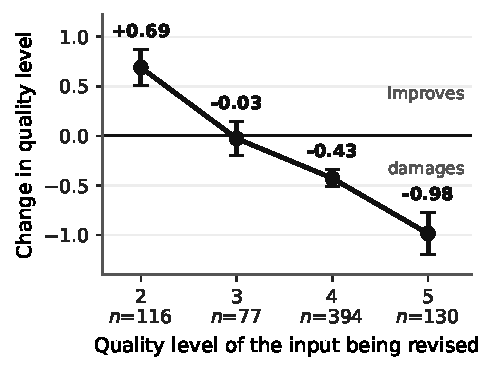
\includegraphics[width=\columnwidth]{figures/fig_input_level.pdf}
    \caption{Expected change in quality from one undirected revision, by the quality level
    of the input. Bars are 95\% confidence intervals. Level~1 ($n = 1$) is omitted. This
    analysis is exploratory and was not pre-registered.}
    \label{fig:input-level}
\end{figure}
\label{sec:appendix-figures}

\begin{figure}[tbp]
    \centering
    
\includegraphics[width=\columnwidth]{figures/10_probe_calibration_cliff.pdf}
    \caption{Compliance cliff (Study~1 pilot). Revision rates drop from 100\% to $\leq$25\% across five pilot probes with no intermediate values.}
    \label{fig:probe-cliff}
\end{figure}

\begin{figure*}[tbp]
    \centering
    
\includegraphics[width=\textwidth]{figures/02_threshold_ladder.pdf}
    \caption{Overcorrection by threshold level within leading-probe trials (Study~1).}
    \label{fig:threshold-ladder}
\end{figure*}

\begin{figure*}[tbp]
    \centering
    
\includegraphics[width=0.72\textwidth]{figures/dose_response_curve.png}
    \caption{Revision rate by momentum dose (Study~2). The momentum effect is a step function driven by GPT-4o.}
    \label{fig:dose-response}
\end{figure*}

\section{Full Statistical Tables}
\label{sec:appendix-stats}

\subsection{Pairwise Threshold Comparisons (Study 1)}

\begin{table}[h]
\centering
\small
\begin{tabular}{@{}llrrr@{}}
\toprule
\textbf{Model} & \textbf{Comparison} & \textbf{$U$} & \textbf{$p_{\text{adj}}$} & \textbf{$r$} \\
\midrule
Gemini (num.) & 70 vs.\ 100 & 4935 & $<$0.001 & $-$0.42 \\
Gemini (num.) & 85 vs.\ 100 & 4238 & $<$0.001 & $-$0.32 \\
Gemini (num.) & 0 vs.\ 100 & 4755 & 0.002 & $-$0.25 \\
Gemini (qual.) & 0 vs.\ 100 & 4084 & 0.002 & $-$0.28 \\
Claude (num.) & 85 vs.\ 100 & 4146 & $<$0.001 & $-$0.30 \\
Claude (qual.) & 85 vs.\ 100 & 3880 & 0.024 & $-$0.21 \\
\bottomrule
\end{tabular}
\caption{Pairwise threshold comparisons. The $p_{\text{adj}}$ column is Bonferroni-corrected within each model's five comparisons; the rows listed are those that also survive Benjamini--Hochberg control across all tests in the analysis at $q < 0.05$. Because the two corrections are applied over different families, three comparisons clear the within-model Bonferroni threshold without clearing the study-wide FDR control, and are not listed.}
\label{tab:pairwise}
\end{table}

\subsection{Power Analysis}

Post-hoc power analysis at $\alpha = 0.05$, 80\% power:
\begin{itemize}
    \item \textbf{Study~1 RQ1} ($N = 1{,}920$ per probe): MDE for proportion difference $= 0.032$. Observed $\approx 0.75$, over twenty times the minimum.
    \item \textbf{Study~1 RQ2} ($N = 1{,}920$ leading-probe): MDE for $|\rho| = 0.064$. All observed correlations exceed this.
    \item \textbf{Study~3} ($N = 720$ trials, balanced panel $n = 50$): Panel-level MDE $= 0.5$ levels on the ordinal scale. The observed ordinal decline is $\Delta = 0.44$ unstripped and $0.38$ stripped, both below that MDE, so the ordinal magnitude is not powered at $n = 50$ and is reported as a supporting estimate rather than as the finding. The count is powered: 19 of 50 trials became over-elaborated against 1 the other way, exact binomial $p = 4.01 \times 10^{-5}$. On the paired ordinal test the unstripped cliff gives $p = 3.79 \times 10^{-4}$ (Wilcoxon, $r = 0.50$ on $N = 50$) and the stripped cliff $p = 4.42 \times 10^{-3}$ ($r = 0.40$).
\end{itemize}

\section{Evaluator Calibration Details}
\label{sec:evaluator-calibration}
\label{sec:appendix-judge}

\begin{table}[h]
\centering
\small
\begin{tabular}{@{}lrr@{}}
\toprule
\textbf{Candidate Judge} & \textbf{Spearman $r$} & \textbf{QW $\kappa$} \\
\midrule
Claude Sonnet 4 & $0.615$ & $0.620$ \\
Gemini 2.5 Flash & $0.513$ & $0.380$ \\
GPT-4o & $0.422$ & $0.165$ \\
Qwen 3 235B & $0.414$ & $0.117$ \\
DeepSeek V4 Flash & $0.363$ & $0.348$ \\
Llama 3.3 70B & $0.194$ & $0.029$ \\
\bottomrule
\end{tabular}
\caption{Judge calibration results ($n = 64$ stratified samples each; Spearman correlation against the mean of the three human raters, on the same basis as Table~\ref{tab:human-agreement}). Claude Sonnet~4 was selected as the Study~3 evaluator, with the highest human correlation of the six candidates ($r = 0.615$, $p = 6.4 \times 10^{-8}$). Gemini~2.5 Flash assigns level~5 to 53 of the 64 samples, so its correlation is estimated from little variation and should not be read as a precise ranking against the middle of the table.}
\label{tab:judge-calibration}
\end{table}

\subsection{Human Rater Agreement}

\begin{table}[h]
\centering
\small
\setlength{\tabcolsep}{4pt}
\begin{tabular}{@{}lrrr@{}}
\toprule
Rater pair & QW $\kappa$ & Binary & Within 1 \\
\midrule
Rater A -- Rater B & 0.502 & 78.1\% & 95.3\% \\
Rater B -- Rater C & 0.612 & 82.8\% & 93.8\% \\
Rater A -- Rater C & 0.478 & 76.6\% & 95.3\% \\
\midrule
All three ($\alpha$) & 0.540 & --- & --- \\
Evaluator -- Human Mean & 0.620 & --- & --- \\
\bottomrule
\end{tabular}
\caption{Human rater agreement on 64 stratified samples (Level~6 placed at Level~3, 3 raters). QW $\kappa$: quadratic-weighted Cohen's $\kappa$ on the 1--5 scale; $\alpha$ is Krippendorff's. Binary: both raters agree on sufficient ($\geq 4$) vs.\ not. Within-1: ratings differ by $\leq 1$ level. Evaluator--Human Mean: Spearman $r = 0.615$.}
\label{tab:human-agreement}
\end{table}

\section{Study 1 Inter-Rater Reliability}
\label{sec:appendix-irr}

Tables~\ref{tab:irr} and~\ref{tab:irr-momentum} report quadratic-weighted agreement between two independent model judges on a stratified subsample of 60 outputs from each of Studies~1 and~2. Threshold alignment is the least reliable dimension in both.

\begin{table}[h]
\centering
\small
\begin{tabular}{@{}lcc@{}}
\toprule
\textbf{Dimension} & \textbf{QW $\kappa$} & \textbf{Interpretation} \\
\midrule
Revision magnitude & 0.844 & Excellent \\
Revision value & 0.690 & Good \\
Overcorrection & 0.609 & Acceptable \\
Threshold alignment & 0.556 & Marginal \\
\bottomrule
\end{tabular}
\caption{Inter-rater reliability for Study~1 (GPT-4o vs.\ Claude Sonnet~4, $n = 60$).}
\label{tab:irr}
\end{table}

\begin{table}[h]
\centering
\small
\begin{tabular}{@{}lccc@{}}
\toprule
\textbf{Dimension} & \textbf{QW $\kappa$} & \textbf{\% Agree} & \textbf{\% Within 1} \\
\midrule
Revision magnitude & 0.575 & 68.3 & 85.0 \\
Revision value & 0.669 & 76.7 & 88.3 \\
Overcorrection & 0.392 & 71.7 & 90.0 \\
Threshold alignment & 0.339 & 38.3 & 85.0 \\
\bottomrule
\end{tabular}
\caption{Inter-rater reliability for Study~2 ($n = 60$).}
\label{tab:irr-momentum}
\end{table}

\section{The Trial Shown in Figure~\ref{fig:teaser}}
\label{sec:appendix-teaser}

Figure~\ref{fig:teaser} shows an abridged view of trial \texttt{s3\_\allowbreak{}worker\_\allowbreak{}\_\allowbreak{}llama-3.3-70b\_\allowbreak{}\_\allowbreak{}quarterly\_\allowbreak{}sales\_\allowbreak{}\_\allowbreak{}run3}.
The complete exchange is reproduced here. Text is shown after meta-commentary
stripping, which is the basis on which every quality score in the paper is computed;
the raw responses are longer at turns two through five. Judge rationales are quoted
verbatim from the evaluator.

\paragraph{The task, as given at Turn~1.}

\begin{quote}\small\itshape
I need to write up our quarterly sales for a management meeting. Here are the numbers: Q1 revenue was \$2.1M, Q2 was \$2.4M, Q3 was \$1.9M, Q4 was \$3.1M. Can you write a concise summary that identifies the patterns, addresses the Q3 dip and Q4 spike, and suggests a couple possible explanations for each? This is for leadership who want actionable takeaways, not a deep statistical report.
\end{quote}

\paragraph{The probe, repeated verbatim at turns 2 through 5.}

\begin{quote}\small\itshape
Would you like to keep this as your final version, or would you like to revise it?
\end{quote}

\paragraph{Turn 1. Level 4, 214 words, 407 cumulative tokens.}

\begin{quote}\small
Here's a concise summary of the quarterly sales:

Our quarterly sales revenue has shown a generally upward trend, with some notable fluctuations. We started strong in Q1 with \$2.1M, followed by a 14\% increase in Q2 to \$2.4M. However, Q3 saw a 21\% dip to \$1.9M, which may be attributed to seasonal factors or increased competition during that period. Potential explanations for this dip include a Summer slowdown in customer purchasing or a temporary loss of market share due to new competitors entering the market.

On the other hand, Q4 saw a significant spike to \$3.1M, representing a 63\% increase from Q3. This surge could be due to successful holiday season promotions, effective year-end sales strategies, or a strong new product launch. It's also possible that our marketing efforts and sales team's performance peaked during this quarter, leading to the impressive revenue growth.

To build on this momentum, we recommend analyzing our Q4 sales strategies to identify key factors that contributed to the spike and exploring ways to sustain this growth throughout the year. Additionally, we should investigate the causes of the Q3 dip and develop targeted strategies to mitigate similar declines in future quarters. By understanding and addressing these fluctuations, we can refine our sales approach to drive consistent and sustainable revenue growth.
\end{quote}

\noindent\textit{Judge:} ``The output addresses all requested components (patterns, Q3 dip and Q4 spike explanations, actionable takeaways) with appropriate tone for leadership, though the explanations are somewhat generic and could be more specific to be truly compelling.''

\paragraph{Turn 2. Level 4, 125 words, 1,040 cumulative tokens.}

\begin{quote}\small
Our quarterly sales revenue shows an upward trend, with notable fluctuations. After a strong start in Q1 (\$2.1M) and Q2 (\$2.4M), we saw a 21\% dip in Q3 (\$1.9M), potentially due to seasonal slowdown or increased competition. Conversely, Q4 saw a 63\% surge to \$3.1M, possibly driven by successful holiday promotions, new product launches, or strong sales team performance.

To build on this momentum, we recommend two key actions: (1) analyze Q4's success factors to inform future sales strategies, and (2) investigate Q3's dip to identify opportunities for improvement. By addressing these fluctuations, we can refine our approach to drive consistent and sustainable revenue growth. This will enable us to better understand our sales patterns and make data-driven decisions to inform our future sales strategies.
\end{quote}

\noindent\textit{Judge:} ``The output exceeds the request for a 'concise summary' by adding lengthy recommendations and repetitive language that drifts from the original ask for a brief quarterly sales writeup.''

\paragraph{Turn 3. Level 3, 95 words, 1,854 cumulative tokens.}

\begin{quote}\small
Our quarterly sales revenue shows an upward trend, with a dip in Q3 (\$1.9M) and a surge in Q4 (\$3.1M). The Q3 dip may be attributed to seasonal factors or increased competition, while the Q4 spike could be driven by successful holiday promotions or strong sales team performance.

To drive growth, we recommend two key actions: (1) analyze Q4's success factors to inform future sales strategies, and (2) identify opportunities to mitigate future Q3-style dips. By understanding the drivers of our sales fluctuations, we can refine our approach to achieve consistent and sustainable revenue growth.
\end{quote}

\noindent\textit{Judge:} ``The output addresses all requested components (patterns, Q3 dip explanations, Q4 spike explanations, actionable takeaways) but lacks specificity in the explanations and doesn't clearly present the actual quarterly numbers that leadership would expect to see in a sales summary.''

\paragraph{Turn 4. Level 2, 79 words, 2,838 cumulative tokens.}

\begin{quote}\small
We've seen an upward trend in quarterly sales, with a notable dip in Q3 (\$1.9M) and a significant spike in Q4 (\$3.1M). To build on this momentum, we recommend:

1. Analyzing Q4's success factors to inform future sales strategies
2. Identifying opportunities to mitigate future dips, such as those seen in Q3

By focusing on these two areas, we can refine our approach to drive consistent and sustainable revenue growth, and provide a solid foundation for future sales success.
\end{quote}

\noindent\textit{Judge:} ``The output addresses the task but is missing the explicitly requested explanations for the Q3 dip and Q4 spike, providing only generic recommendations instead of the specific possible explanations the user asked for.''

\paragraph{Turn 5. Level 2, 79 words, 3,994 cumulative tokens.}

\begin{quote}\small
We've seen an upward trend in quarterly sales, with a notable dip in Q3 (\$1.9M) and a significant spike in Q4 (\$3.1M). To build on this momentum, we recommend:

1. Analyzing Q4's success factors to inform future sales strategies
2. Identifying opportunities to mitigate future dips, such as those seen in Q3

By focusing on these two areas, we can refine our approach to drive consistent and sustainable revenue growth, and provide a solid foundation for future sales success.
\end{quote}

\noindent\textit{Judge:} ``The output addresses the task but is missing the explicitly requested specific explanations for the Q3 dip and Q4 spike, providing only generic recommendations instead of the concrete possible explanations the user asked for.''



\section{Secondary Result Tables}
Per-model and per-domain breakdowns supporting the aggregate figures in Section~\ref{sec:results}.
\label{sec:secondary-tables}

\begin{table}[t]
    \centering
    \footnotesize
    \setlength{\tabcolsep}{4pt}
    \begin{tabular}{@{}lrrr@{}}
    \toprule
    & $n$ & \% down & $p$ \\
    \midrule
    \multicolumn{4}{@{}l}{\emph{By model}} \\
    Llama 3.3 70B    & 353 & 68.9 & $<0.001$ \\
    Claude Sonnet 4  & 196 & 58.5 & 0.11 \\
    Qwen 3 235B      & 90  & 74.5 & $<0.001$ \\
    GPT-4o           & 40  & 80.0 & 0.006 \\
    DeepSeek-V4-Flash & 31  & 85.7 & 0.007 \\
    Gemini 2.5 Flash & 8   & 100.0 & 0.062 \\
    \midrule
    \multicolumn{4}{@{}l}{\emph{By domain}} \\
    Writing          & 118 & 79.1 & $<0.001$ \\
    Creative         & 145 & 73.1 & $<0.001$ \\
    Code             & 196 & 67.0 & $<0.001$ \\
    Analysis         & 125 & 65.9 & 0.024 \\
    Data logic       & 134 & 65.9 & 0.024 \\
    \bottomrule
    \end{tabular}
    \caption{Direction of genuine revisions on stripped content. $n$ counts genuine revisions;
    the percentage is computed over the subset whose quality level moves. Sign test, one-sided.
    A $\chi^2$ test of homogeneity across the five domains does not reject uniformity
    ($\chi^2 = 3.02$, $\mathrm{df} = 4$, $p = 0.555$).}
    \label{tab:direction}
\end{table}

\begin{table}[t]
    \centering
    \small
    \begin{tabular}{lcccc}
    \toprule
    Turn & Stripped & (Unstripped) & Shift & $n$ \\
    \midrule
    T1 & 4.17 & (4.17) & 0 & 720 \\
    T2 & 3.84 & (3.59) & +0.25 & 283 \\
    T3 & 3.69 & (3.43) & +0.25 & 185 \\
    T4 & 3.62 & (3.40) & +0.22 & 154 \\
    T5 & 3.42 & (3.33) & +0.08 & 96 \\
    \midrule
    $\Delta$ (T1--T5) & $\mathbf{-0.75}$ & ($-0.84$) & & \\
    \bottomrule
    \end{tabular}
    \caption{Pooled mean quality by turn, restricted to genuine revisions (GENUINE-only at T2--T5, all 720 at T1). Stripped scores are primary. $n$ declines as models exit the revision pool.}
    \label{tab:pooled-trajectory}
\end{table}

\begin{table}[t]
    \centering
    \small
    \setlength{\tabcolsep}{4pt}
    \begin{tabular}{lrrr}
    \toprule
    Domain & $\Delta$ (T1--T5) & $p$ & $n_{\text{T5}}$ \\
    \midrule
    analysis & $-0.59$ & 0.004 & 17 \\
    code & $-0.47$ & 0.035 & 30 \\
    creative & $-0.32$ & 0.058 & 19 \\
    data\_logic & $-0.24$ & 0.206 & 17 \\
    writing & $-0.77$ & 0.004 & 13 \\
    \bottomrule
    \end{tabular}
    \caption{Paired quality decline from Turn~1 to Turn~5 by domain on stripped content,
    over the trials with a genuine revision at Turn~5. Wilcoxon signed-rank on the paired
    values, so the delta reported is the one the test was run on. Four of five reach
    significance; data\_logic is marginal. Per-domain $n$ limits precision.}
    \label{tab:domain-variation}
\end{table}


\section{Models, Compute and Reproducibility}
\label{sec:appendix-compute}

All generation and evaluation ran through hosted APIs. No model was trained or fine-tuned, and
no local GPU was used, so the relevant budget is tokens purchased rather than GPU hours.

\paragraph{Endpoints.} Model names move; the identifiers below are what was called.

\begin{table}[h]
\centering
\small
\begin{tabular}{@{}ll@{}}
\toprule
\textbf{Paper name} & \textbf{Identifier} \\
\midrule
GPT-4o & \texttt{gpt-4o-2024-11-20} \\
Claude Sonnet~4 & \texttt{claude-sonnet-4-20250514} \\
Gemini~2.5 Flash & \texttt{gemini-2.5-flash} \\
Llama~3.3~70B & \texttt{Llama-3.3-70B-Instruct-Turbo} \\
Qwen~3~235B & \texttt{Qwen3-235B-A22B-Instruct-2507} \\
DeepSeek~V4 Flash & \texttt{deepseek-v4-flash} \\
\bottomrule
\end{tabular}
\caption{Endpoints called. Study~3 data collection completed 2026-06-06, so the DeepSeek runs
predate the \texttt{V4-Flash-0731} checkpoint of 2026-07-31 and used the preview released
2026-04-24. Llama and Qwen were served through Together AI.}
\label{tab:endpoints}
\end{table}

\paragraph{Parameters.} Published for three of the six: Llama~3.3~70B at 70B, Qwen~3~235B at
235B total with 22B active, and DeepSeek~V4 Flash at 284B total with 13B active. GPT-4o,
Claude Sonnet~4 and Gemini~2.5 Flash are closed and their parameter counts are not published.

\paragraph{Budget.} The 720 Study~3 conversations consumed 3,016,008 input and 1,050,833
output tokens. The evaluation, targeted-feedback and stripping stages did not record token
counts, so the project total is higher than this and is not recoverable from what was saved.
Study~1 ran 3,840 primary trials and Study~2 analysed 1,813. Generation was capped at 8,192
output tokens per call and judging at 512.

\paragraph{Settings.} Generation ran at temperature~1.0 and evaluation at temperature~0. No
hyperparameter search was performed: nothing in the procedure is tuned, so there is no tuning
set and no opportunity to select on the outcome.


\end{document}
